\subsubsection{UC31 - Visualizzazione errore nome dizionario dati}\label{UC31}

\begin{figure}[H]
  \centering
  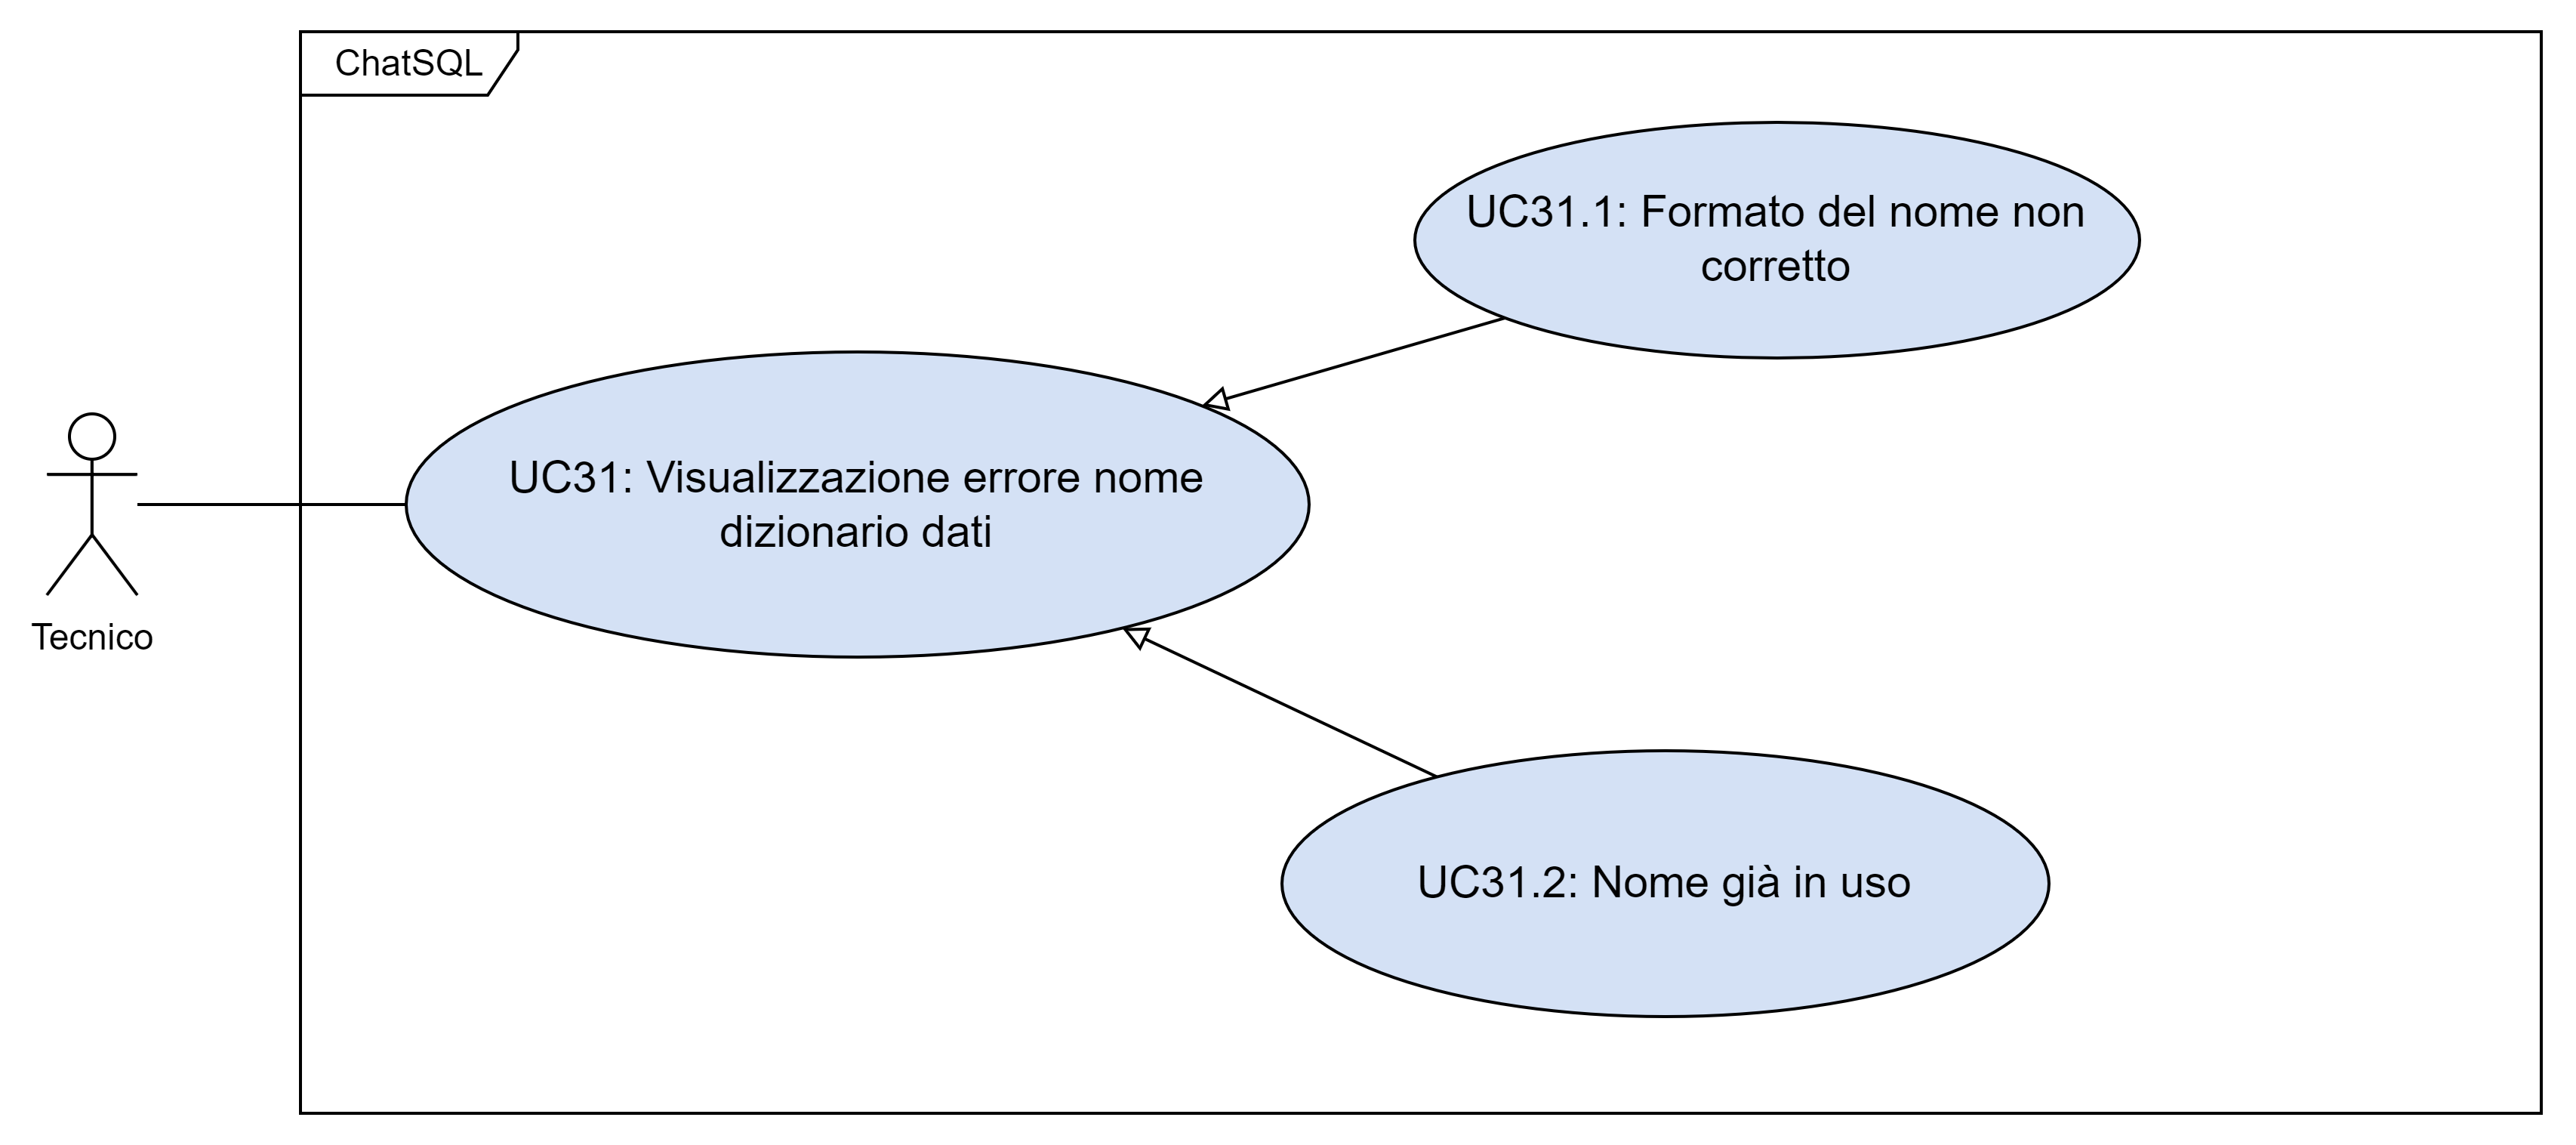
\includegraphics[width=0.90\textwidth]{assets/uc31.png}
  \caption{UC31}
\end{figure}

\paragraph*{Descrizione}
Nel caso cui il sistema riscontri delle anomalie nella validazione del nome di un \glossario{dizionario dati}, il Tecnico visualizza un messaggio d'errore.

\paragraph*{Attori principali}
Tecnico

\paragraph*{Precondizioni}
\begin{itemize}
  \item Il Tecnico ha richiesto il salvataggio o la modifica di un \glossario{dizionario dati} nel sistema;
  \item Il nome del \glossario{dizionario dati} non è valido.
\end{itemize}

\paragraph*{Postcondizioni}
\begin{itemize}
  \item Viene visualizzato un messaggio d'errore esplicativo.
\end{itemize}

\paragraph*{Scenario principale}
\begin{enumerate}
  \item Il sistema riscontra un errore nella validazione del nome del \glossario{dizionario dati};
  \item Il sistema restituisce un messaggio con i dettagli dell'errore.  
\end{enumerate}

\paragraph*{Specializzazioni}
\begin{itemize}
  \item Formato del nome non corretto (\hyperref[UC39]{UC39});
  \item Nome già in uso (\hyperref[UC40]{UC40}).
\end{itemize}
